\section{Pre-amplifier}
In order to transfer as much signal from the guitar as possible, and avoid some significant voltage division between the guitar and the \gls{dsp} in some frequency area, a \gls{preamp} will be designed. The output impedance of the guitar is measured and the result is shown in \autoref{app:output_impedance}. This shows that the output impedance for a guitar is not the same from \SI{10}{\hertz} to \SI{22}{\kilo\hertz} and the output impedance is generally very high. Therefore the \gls{preamp} needs to have an very high input impedance to avoid significant voltage division in the frequency area from \SI{10}{\kilo\hertz} to \SI{22}{\kilo\hertz} compared to the frequency area from \SI{10}{\hertz} to \SI{10}{\kilo\hertz}. The input impedance shall therefore be much higher than \SI{73.06}{\kilo\hertz} which is the highest measured output impedance on the guitar, to allow as much signal transfer as possible.

\subsection{Component chose}

As seen in the \autoref{app:guitar_max_amplitude} that the maximum output signal peak amplitude from the guitar is about $\SI{1}{\volt}_{peak}$ and the 
\gls{dsp} have a capasitivity of maximum $\SI{0.5}{\volt}_{RMS}$ which give a peak value of $\SI{0.707}{\volt}_{peak}$. To make a general \gls{preamp} that works with more guitar than only the measured guitar, the \gls{preamp} will be designed with a volume control. The \gls{preamp} shall have a voltage gain of approximate \SI{6}{\decibel} and the input impedance shall be over a decade higher than the guitar output impedance. The \gls{preamp} will be designed to fit intro a \SI{6.33}{\milli\meter}  jack connector house, and therefore the chosen \gls{opamp} is the smallest in komponenten at Aalborg University. The chosen \gls{opamp} is ST ts424 \citep{TS464} and the \gls{preamp} will be designed to fit this \gls{opamp}. 
	An \gls{opamp} often have an input impedance of more than \SI{1}{\mega\ohm} and have a gain of about \SI{100}{\decibel}, and after the feedback circuit is implemented on the \gls{opamp} the input impedance is even higher and the output impedance is even lower. A simple diagram over the \gls{preamp} is shown in \autoref{fig:simple_preamp} 

\begin{figure}[h!]
\centering
\begin{circuitikz}\draw (0,0)
(0,0)to[short, o-]node[left,above]{$Input$}(1,0)
to[amp, t=$G1$]  (3,0)
to[short] (3,0)
to[pR=$ $](3,-2)
to[short](3,-2)node[ground]{}(3.5,-1)
to[short] (4,-1)
to[short] (4,0)
to[amp, t=$G2$]  (6,0)
(6,0)to[short, -o]node[left,above]{$Output$}(7,0)
%to[short] (0,0)
;\end{circuitikz}
\caption{A simple block diagram of the \gls{preamp}}
\label{fig:simple_preamp}
\end{figure}


\subsection{Design of $G1$ resistor}
The \gls{opamp} part $G1$ in \autoref{fig:simple_preamp} can ether be working in non inverting or inverting \gls{opamp} configuration, but since the \gls{preamp} shall have a gain of \SI{6}{\decibel} and a high input impedance, the non inverting \gls{opamp} configuration will fit very well, because it is a Voltage-seriel feedback configuration. The seriel feedback configuration means that the input impedance is higher than a parallel feedback, because the feedback circuit is in seriel with the input imperdance of the \gls{opamp} The schematics of a non inverting \gls{opamp} is shown in the following schematic \autoref{fig:preamp_opamp}

\begin{figure}[h!]
\centering
\begin{circuitikz}\draw (0,0)
node[op amp,yscale=-1] (opamp) {} 
(-3,-3.5)
to[R=$R_{Bias}$] (-3,0.5)
to[short](opamp.+) 
(-5,0.5)to[short, o-]node[left,above]{$Input$} (-3,0.5)
(opamp.-) 
(opamp.out) 
to[short] (2,0)
to[short] (2,-1.5)
to[R=$R_F$] (-1.5,-1.5)
to[short] (-1.5,-0.5)
to[short] (-1,-0.5)
(-1.5,-1.5)to[R=$R_1$] (-1.5,-3.5)
(2,-1.5)to[pR, l_=$R_V$] (2,-3.5)
(2.5,-2.5)to[short, -o]node[left,above]{$Output$} (4,-2.5)
(-3,-3.5)to[short](2,-3.5)
(-1.5,-3.5)to[V=$V_{Offset}$] (-1.5,-5)node[ground]{}(-1.5,-5.5)
;\end{circuitikz}
\caption{The schematic over $G1$, see \autoref{fig:simple_preamp}}
\label{fig:preamp_opamp}
\end{figure}

The output is looking into $G2$ which is a \gls{opamp} in buffer circuit with over \SI{1}{\mega\ohm}, so the calculation is without the $G2$ \gls{opamp} The calculation is also without the $V_{Offset}$ power supply, because a voltage power supply is a short circuit with respect to impedances.  The equivalent schematic of a non inverting \gls{opamp} is as following \autoref{fig:preamp_opamp_equa}

\begin{figure}[h!]
\centering
\begin{circuitikz}\draw (0,0)
to[R=$R_{Bias}$] (0,-2)node[ground]{}(0,-2.5)
(0,0)to[R=$Z_{i}$] (2,0)
to[R=$Z_{i\beta}$] (4,0)
to[V=$\beta \cdot V_o$] (4,-2)node[ground]{}(4,-2.5)
(0,0)to[short, -o]node[left,above]{$Z_{Input}$} (-3,0)
;\end{circuitikz}
\caption{The equivalent input impedance schematic of $G1$, see \autoref{fig:simple_preamp}}
\label{fig:preamp_opamp_equa}
\end{figure}

\newpage

Calculating of $Z_{i\beta}$ is done by following \autoref{eq:preamp_ib}

\begin{equation}\label{eq:preamp_ib}
        Z_{i\beta} = R_F\parallel R_1
        \addunit{\si{\ohm}}
    \end{equation}

    \startexplain
        \explain{$R_1$ is a resistor in the feedback circuit}{\si{\ohm}}
        \explain{$R_F$ is a resistor in the feedback circuit}{\si{\ohm}}
        \explain{$Z_{i\beta}$ the impedance of the feedback circuit}{\si{\ohm}}
    \stopexplain

Calculating of $\beta$ is done by following \autoref{eq:preamp_beta}

\begin{equation}\label{eq:preamp_beta}
        \beta = \frac{R_1}{R_1 + R_F}
        \addunit{\si{1}}
    \end{equation}
    \startexplain
        \explain{$\beta$ is the feedback factor}{\si{1}}
    \stopexplain


The resulting input impedance of the \gls{preamp} will be as following \autoref{eq:preamp_result}.

\begin{equation}\label{eq:preamp_result}
        Z_{In_{G1}} = R_{Bias}\parallel (Z_i + Z_{i \beta}) \cdot (1+\beta \cdot A) \simeq R_{Bias}
        \addunit{\si{\ohm}}
    \end{equation}

    \startexplain
        \explain{$Z_{In_{G1}} $ is the resulting input impedance of $G1$}{\si{\ohm}}
        \explain{$R_{Bias}$ An bias resistor}{\si{\ohm}}
        \explain{$Z_i$ The input impedance of the \gls{opamp}}{\si{\ohm}}
         \explain{$A$ is the gain of the \gls{opamp}}{\si{1}}
    \stopexplain

The feedback circuit will increase the $Z_{i}$ by a factor of $(1+\beta \cdot A)$, and since the input impedance of an \gls{opamp} is over \SI{1}{\mega\ohm}, and the feedback circuit will decrease the output impedance by a factor of $(1+\beta \cdot A)$, the feedback resistors value dose not matters at all, only the factors matters. The following circuit \autoref{fig:preamp_opamp_equa_out} shows the output impedance equivalent circuit of the \gls{opamp}

\begin{figure}[h!]
\centering
\begin{circuitikz}\draw (0,0)
to[V=$A \cdot V_i$] (0,-3)
(0,0)to[R=$Z_o$](2,0)
to[R=$Z_{o\beta}$](2,-3)
(2,0)to[short](4,0)
(4,0)to[pR, l_=$R_V$](4,-3)
(0,-3)to[short, -o](6,-3)
(4.5,-1.5)to[short, -o](6,-1.5)
;\end{circuitikz}
\caption{The equivalent output impedance schematic of $G1$, see \autoref{fig:simple_preamp}}
\label{fig:preamp_opamp_equa_out}
\end{figure}


Calculating of $Z_{o\beta}$ is done by following \autoref{eq:preamp_beta_out}

\begin{equation}\label{eq:preamp_beta_out}
        Z_{o\beta} = R_F+R_1
        \addunit{\si{\ohm}}
    \end{equation}

A voltage power supply is a short cut with respect to impedance, so the resulting output impedance of $G1$ is calculated by following \autoref{eq:preamp_zout_out} 

\begin{equation}\label{eq:preamp_zout_out}
        Z_{out_{G1}} = \frac{ Z_{o\beta} \parallel Z_{o} }{1+\beta \cdot A'}
        \addunit{\si{\ohm}}
    \end{equation}
    \startexplain
        \explain{$A' =A \cdot \frac{Z_{o\beta}}{Z_o+Z_{o\beta}}$ which is the voltage division between $Z_{o\beta}$ and $Z_{o}$ multiplied by $A$ }{\si{1}}
\explain{$Z_{out_{G1}}$ is the total output impedance of $G1$ }{\si{\ohm}}
    \stopexplain

The $R_V$ is chosen to \SI{10}{\kilo\ohm} to make as small voltage division between $Z_{out}$ and $R_V$ as possible. In another way, to keep the voltage over $Z_{out_{G1}}$ as small as possible. The $R_F$ is chosen to be \SI{5}{\kilo\ohm}


The approximated amplification of a non inverting \gls{opamp} is given by \autoref{eq:preamp_amplification}

\begin{equation}\label{eq:preamp_amplification}
        G =1+\frac{R_F}{R_1}
        \addunit{\si{1}}
    \end{equation}

    \startexplain
        \explain{$G$ is the amplification of $G1$}{\si{1}}
    \stopexplain

Then  $R_1$ is founded to \SI{5}{\kilo\ohm} by isolate $R_1$ in the above \autoref{eq:preamp_amplification}.
 
   
 \subsection{Design of $G1$ DC offset}
  
  Designing of the voltage offset power supply will be done by two resistors which divide the voltage by two equals, and afterwards an \gls{opamp} in buffer circuit is used to make a small output impedance. Because the \gls{opamp} have a impedance of more than \SI{1}{\mega\ohm} the resistor size does not matte at all, but a non ideal \gls{opamp} do have a bias current in the input, that will affect the division if the resistors is to large. To keep the division approximate by two, the resistors shall be at leas a decade smaller than the input impedance of the \gls{opamp}. The voltage offset power supply circuit is designed as following \autoref{fig:preamp_voffset}.
    
  \begin{figure}[h!]
\centering
\begin{circuitikz}\draw (0,0)
node[op amp,yscale=-1] (opamp) {} 
(-9,0.5)to[short, o-]node[right,above]{$V_s$} (-8,0.5)
to[R=$R_{2}$]
(-5,0.5)to[C=$C_{Offset}$](-5,-2)node[ground]{}
(-5,0.5)to[short]
(-3,0.5)to[R=$R_{Offset}$](-3,-2)node[ground]{}
(opamp.+) 
(-3,0.5)to(opamp.+) 
(opamp.out) 
to[short] (2,0)
to[short] (2,-1.5)
to[short] (-1.5,-1.5)
to[short] (-1.5,-0.5)
to[short] (-1,-0.5)
(2,0)to[short, -o] (4,-0)node[left,above]{$V_{Offset}$}
;\end{circuitikz}
\caption{The offset power supply to $G1$, see \autoref{fig:preamp_opamp} }
\label{fig:preamp_voffset}
\end{figure}
  
Where $C_{Offset}$ is used to stabilize the voltage at the input of the \gls{opamp} and the calculating of $R_{Offset}$ and $R_{2}$ is done as following \autoref{eq:preamp_offset}

\begin{equation}\label{eq:preamp_offset}
        R_{Offset} = R_{2} = \frac{Z_{in}}{10}
        \addunit{\si{\ohm}}
    \end{equation}

    \startexplain
        \explain{$Z_{in}$ is the input impedance of the \gls{opamp}}{\si{\ohm}}
        \explain{$R_2$ is the upper resistor in the voltage division circuit}{\si{\ohm}}
        \explain{$R_{offset}$ is the lower resistor in the voltage division circuit}{\si{\ohm}}
    \stopexplain
    
\subsection{Design of input and output DC blocking}

The total circuit of the \gls{preamp} is as \autoref{fig:preamp_total} and the design of $G1$ input capacitor $C_{In}$ and  $G2$ output capacitor $C_{Out}$ will be done beneath the full circuit \autoref{fig:preamp_total}.

\begin{figure}[h!]
\centering
\begin{circuitikz}\draw 
(-5,0.5) node[anchor=south] {$S_{In}$}
(-5,-5.5) node[anchor=south] {$V_{in}$}
(8.5,-3) node[anchor=south] {$S_{Out}$}
(0,0)node[op amp,yscale=-1] (opamp1) {} 
(-3,-3.5)
to[R=$R_{Bias}$] (-3,0.5)
to[short](opamp1.+) 
(-5,0.5)to[C=$C_{In}$, o-] (-3,0.5)
(opamp1.-) 
(opamp1.out) 
to[short] (2,0)
to[short] (2,-1.5)
to[R=$R_F$] (-1.5,-1.5)
to[short] (-1.5,-0.5)
to[short] (-1,-0.5)
(-1.5,-1.5)to[R=$R_1$] (-1.5,-3.5)
(2,-1.5)to[pR, l_=$R_V$] (2,-3.5)
(2.5,-2.5)to[short](4,-2.5)
(-3,-3.5)to[short](2,-3.5)
(5,-3) node[op amp,yscale=-1] (opamp2) {} 
(opamp2.-) 
(opamp2.+) 
(opamp2.out) 
to[short] (7,-3)
to[short] (7,-4.5)
to[short] (3.5,-4.5)
to[short] (3.5,-3.5)
to[short] (4,-3.5)
(7,-3)to[C=$C_{Out}$, -o](8.5,-3)
(2,-6)node[op amp,yscale=-1] (opamp3) {} 
(-5,-5.5)to[R=$R_{2}$, o-]
(-3,-5.5)to[C=$C_{Offset}$](-3,-7.5)node[ground]{}
(-3,-5.5)to[short]
(-1,-5.5)to[R=$R_{Offset}$](-1,-7.5)node[ground]{}
(opamp3.+) 
(-1,-5.5)to(opamp3.+) 
(opamp3.out) 
to[short] (4,-6)
to[short] (4,-7.5)
to[short] (0.5,-7.5)
to[short] (0.5,-6.5)
to[short] (1,-6.5)
(4,-6) to[short] (4,-5)
to[short] (2,-5)
to[short] (2,-3.5)
;\end{circuitikz}
\caption{The full schematic of the \gls{preamp}, $G1$ and $G2$, see \autoref{fig:simple_preamp}}
\label{fig:preamp_total}
\end{figure}

The $C_{In}$ and $Z_{In}$ shall be designed to have an cross frequency of a decade beneath the audibility area. This result in a cross frequency of \SI{2}{\hertz}. The calculating of $C_{In}$ is done by following \autoref{eq:preamp_cin}.

\begin{equation}\label{eq:preamp_cin}
        C_{In} \geq  \frac{1}{2 \pi \cdot Z_{In_{G1}} \cdot f}
        \addunit{\si{\farad}}
    \end{equation}

    \startexplain
         \explain{$C_{In}$ is the Input capacitor}{\si{\farad}}
        \explain{$Z_{In}$ is the input impedance of $G1$}{\si{\ohm}}
        \explain{$f$ is the cross frequency}{\si{\hertz}}
    \stopexplain
    
    The $C_{Out}$ and $Z_{In,\gls{dsp}}$ shall be designed to have an cross frequency of a decade under the audibility area, which will result in a cross frequency of \SI{2}{\hertz}. The calculating of $C_{Out}$ is done by following \autoref{eq:preamp_cout}.

\begin{equation}\label{eq:preamp_cout}
        C_{In} \geq  \frac{1}{2 \pi \cdot Z_{In,\gls{dsp}} \cdot f}
        \addunit{\si{\farad}}
    \end{equation}

    \startexplain
     \explain{$C_{Out}$ is the output capacitor}{\si{\farad}}
        \explain{$Z_{Out}$ is the output impedance of $G2$}{\si{\ohm}}
 \explain{$f$ is the cross frequency}{\si{\hertz}}
    \stopexplain
    
 The $C_{Offset}$ is selected to be separated intro one \SI{100}{\nano\farad} and one \SI{1}{\micro\farad} capacitors.
 
\subsection{\gls{pcb} layout} 
The signal cable will have a capacitive effect on the signal, form the guitar to the \gls{preamp}, and this will cause a low pass filter. In order to avoid the low pass problem with the cable, the \gls{preamp} will be designed to fit inside a \SI{6.35}{\milli\meter} Jack connector house. The chosen Jack connector is ?? and this require a \gls{pcb} with the maximum size of  \SI{1}{\centi\meter} times \SI{2.5}{\centi\meter}. The used cable from the \gls{dsp} to the \gls{preamp} is a balanced cable, where the shield is used as ground to both signal and power. The red wire is used as signal wire and the black wire is used as positive power wire. The resulting \gls{preamp} layout is as following \autoref{fig:preamp_layout}
 
 \begin{figure}[h]
	\centering
		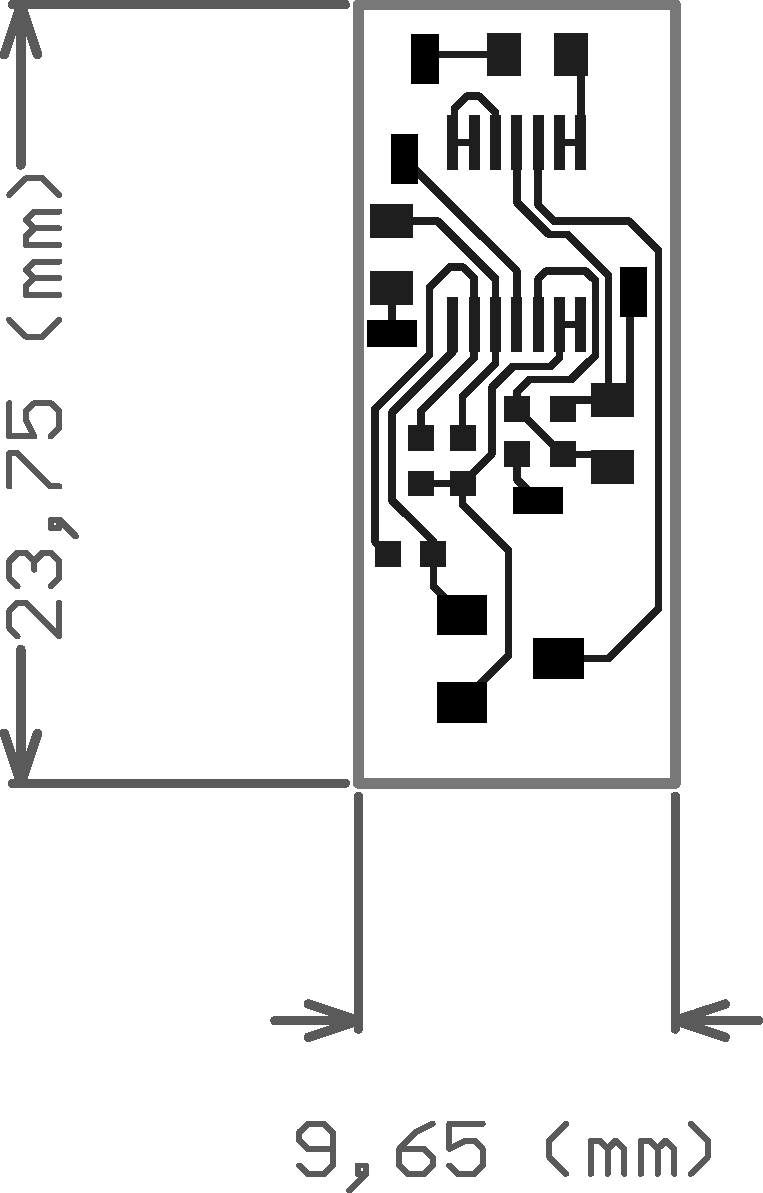
\includegraphics[width=0.2\textwidth]{PreAmp.pdf}
		\caption{The \gls{preamp} layout}
		\label{fig:preamp_layout}
\end{figure}
 